\documentclass[11pt]{article}
\usepackage{../style/forage}

% Figures and tables in figures/ are generated by analysis.ipynb.
% Re-run the notebook if the data changes, then recompile.

\begin{document}

% ================= Title page =================
\begin{titlepage}
  \vspace*{4cm}
  {\color{navy}\fontsize{30}{36}\selectfont Market Insight Report}\par\medskip
  {\Large Rising Rates, Volatility and Sector Rotation:\\
  Implications for a Technology--Healthcare Portfolio}\par
  {\color{rulegray}\rule{\linewidth}{0.6pt}}\par\bigskip
  \begin{tabular}{@{}ll}
    \textbf{Client:}      & Emerald Investments \\
    \textbf{Prepared by:} & Thiziri Amezza, Sales and Trading Analyst \\
    \textbf{Team:}        & Global Markets Advisory \\
    \textbf{Date:}        & \today \\
  \end{tabular}
  \vfill
  {\small\color{gray}Prepared as part of the Bank of America Global Markets
  Sales and Trading job simulation (Forage). Hypothetical client and data.
  All figures and tables are reproducible with \texttt{analysis.ipynb}.}
\end{titlepage}

% ================= Executive summary =================
\heading{Executive Summary}
Over the seven weeks analysed, interest rates rose by 50 basis points (1.5\%
to 2.0\%) and a cluster of events --- a rate hike announcement, geopolitical
tension and technology earnings --- pushed the VIX from 18 to a peak of 25
before it eased back to 20. Technology, which represents half of Emerald
Investments' portfolio, absorbed most of the shock: it fell for three
consecutive weeks (a 2.3\% drawdown) before recovering on a strong earnings
season. Healthcare did exactly what the client expects of it, posting only one
marginally negative week.

The key finding is one of \textbf{concentration}: with 50\% of the capital,
technology generates about \textbf{91\% of the portfolio's risk}. We recommend
(1) trimming technology from 50\% to 40\% into the current recovery,
(2) keeping healthcare at 30\% as the defensive core, (3) adding financials
(10\%) and a small energy position (5\%) that behaves as a natural hedge against
rising rates, and (4) keeping 15\% in cash with clear rules to buy technology
on future sell-offs. On the same data, this mix delivers a slightly higher
return with \textbf{14\% lower volatility} and a \textbf{32\% smaller maximum
drawdown} --- consistent with the client's goal of long-term growth with
controlled short-term volatility.

\infobox{\faClipboardList}{Client at a glance}{
  \item \textbf{Allocation:} Technology 50\%, Healthcare 30\%, Cash 20\%.
  \item \textbf{Objectives:} long-term growth; mitigate short-term volatility.
  \item \textbf{Risk tolerance:} moderate \quad \textbf{Horizon:} 5--10 years.
  \item \textbf{Key concerns:} tech volatility, rate sensitivity, market and
  geopolitical risk.
}

% ================= Key trends =================
\heading{Key Trends Identified}

\begin{center}
  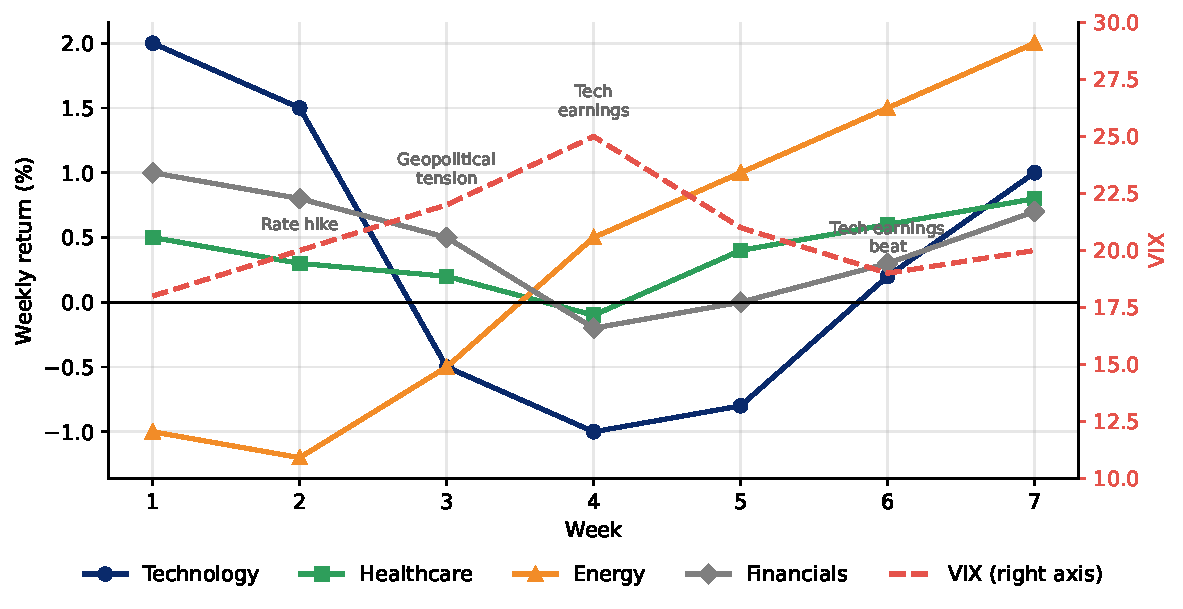
\includegraphics[width=\linewidth]{figures/fig1_returns_vix.pdf}\par
  {\small\color{gray}Figure 1 --- Weekly sector returns (left axis) and VIX
  (right axis, dashed red). Source: simulation sample dataset.}
\end{center}

\begin{center}
  \small\begin{tabular}{@{}lrrrrrrr@{}}
\toprule
Sector & Avg.\ weekly & Std.\ dev. & Cumulative & Worst & Return / & Corr.\ with & Corr.\ with \\
       & return (\%) & (\%) & 7 weeks (\%) & week (\%) & risk & VIX & rate \\
\midrule
Technology & 0.34 & 1.18 & 2.38 & \textminus{}1.00 & 0.29 & \textminus{}0.78 & \textminus{}0.24 \\
Healthcare & 0.39 & 0.29 & 2.73 & \textminus{}0.10 & 1.32 & \textminus{}0.81 & 0.55 \\
Energy & 0.33 & 1.25 & 2.27 & \textminus{}1.20 & 0.26 & 0.08 & 0.96 \\
Financials & 0.44 & 0.44 & 3.14 & \textminus{}0.20 & 1.02 & \textminus{}0.76 & \textminus{}0.32 \\
\bottomrule
\end{tabular}\par\smallskip
  {\color{gray}Table 1 --- Summary statistics, weeks 1--7. ``Return / risk''
  is the average weekly return divided by its standard deviation.}
\end{center}

\subheading{1. Interest rates: a steady tightening cycle}
Rates rose from 1.5\% to 2.0\% over the period, increasing in every week except
week 3 (Figure 2). The move was triggered by the rate hike announcement in week
2 and continued without pause afterwards, which suggests markets should expect
rates to stay higher for longer rather than a one-off adjustment. Higher rates
raise borrowing costs and reduce the present value of future earnings, which
weighs most on growth companies --- the core of the client's technology
holdings.

\begin{center}
  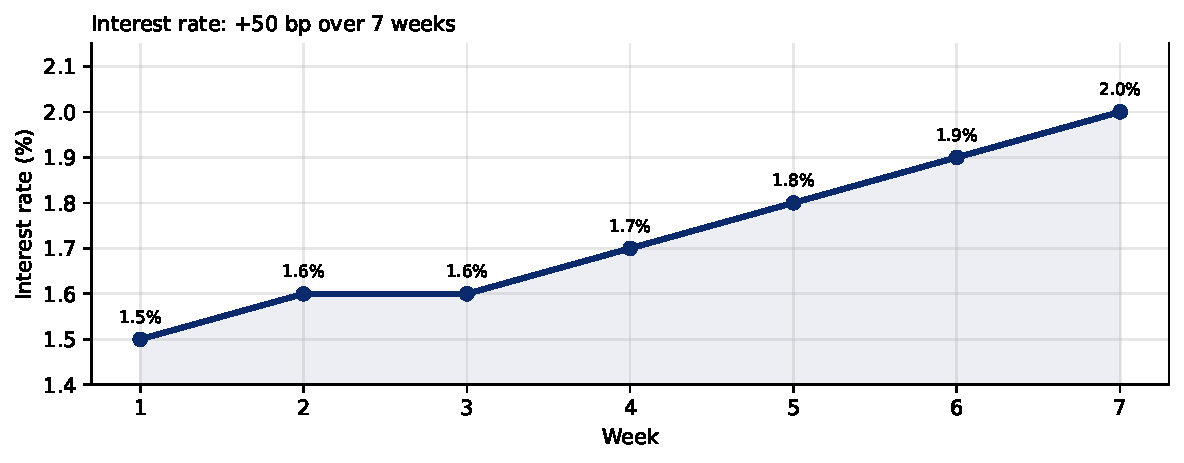
\includegraphics[width=0.85\linewidth]{figures/fig2_interest_rate.pdf}\par
  {\small\color{gray}Figure 2 --- Interest rate path over the period.}
\end{center}

\subheading{2. Volatility: an event-driven spike, not a regime change}
The VIX climbed from 18 to 25 in four weeks as the rate hike (week 2),
geopolitical tension (week 3) and technology earnings (week 4) arrived back to
back, and market sentiment turned from positive to negative. It then fell back
to 19--20 as earnings beat expectations (week 6) and a new government policy
(week 7) restored confidence. The spike was therefore driven by identifiable
events and faded within three weeks --- a pattern that rewards investors who
have a plan and liquidity ready, rather than those who react after the fact.
All sectors except energy moved inversely to the VIX (correlations between
\textminus0.76 and \textminus0.81), so diversification across the client's current sectors
offered little protection at the peak of the stress.

\subheading{3. Sector performance: four very different profiles}
\begin{itemize}[leftmargin=1.5em, itemsep=2pt]
  \item \textbf{Technology --- high return, high risk.} The strongest start
  (+2.0\%, +1.5\%), followed by the sharpest decline (\textminus0.5\%, \textminus1.0\%,
  \textminus0.8\%; a 2.3\% peak-to-trough drawdown) and a recovery after the week 6
  earnings beat. It ends the period up 2.4\%, but with the second-highest
  volatility (1.18\% per week) and the second-lowest return per unit of risk
  (0.29).
  \item \textbf{Healthcare --- the stabiliser.} A similar total return (+2.7\%)
  with four times less volatility (0.29\%). Its only negative week was a
  marginal \textminus0.1\% at the peak of the VIX, and it gained 0.4\% in the week of
  the healthcare regulation news. Best return per unit of risk (1.32).
  \item \textbf{Financials --- best total return.} +3.1\% over the period, with
  low volatility (0.44\%) and a worst week of only \textminus0.2\%. Second-best return
  per unit of risk (1.02).
  \item \textbf{Energy --- a rate-linked recovery.} The weakest start (\textminus1.0\%,
  \textminus1.2\%) followed by five consecutive weekly improvements to +2.0\% in week 7. Its
  performance tracked interest rates almost perfectly (correlation 0.96) and
  was unrelated to the VIX (0.08). Note that energy also fell (\textminus0.5\%) in the
  week of geopolitical tension: its strength in this period came from the rate
  and growth environment, not from geopolitical events.
\end{itemize}

% ================= Portfolio implications =================
\heading{Portfolio Implications}

\subheading{Technology (50\%): the main source of risk}
Technology delivered growth, but it is also where almost all of the risk sits:
because it is four times as volatile as healthcare, it accounts for about
\textbf{91\% of the portfolio's risk} while holding 50\% of the capital. In the
worst week (week 4) the portfolio lost 0.52\%, almost entirely because of
technology. If rates keep rising --- as the trend suggests --- the sector will
remain exposed to further valuation pressure and earnings disappointments. For
a client with a \emph{moderate} risk tolerance and an explicit concern about
overexposure to technology, this concentration is the main issue to address.
The long-term growth case for technology remains intact, so the answer is to
size the position better, not to exit it.

\subheading{Healthcare (30\%): the defensive role is confirmed}
Healthcare held up during the volatile weeks 3--5 and was not hurt by the
regulation news. This directly answers the client's question: yes, healthcare
can balance risk when technology declines. Its low volatility also means it
contributes less than 10\% of total portfolio risk. The current allocation is
appropriate and should be maintained.

\subheading{Cash (20\%): flexibility with a cost}
Cash protected the portfolio during the drawdown and, with rates now at 2.0\%,
earns more than it did at the start of the period. However, over the seven
weeks it earned roughly 0.2\%, against 2--3\% for every equity sector: holding
a fifth of the portfolio in cash has a real opportunity cost for a growth
objective. Some of this reserve can be put to work while keeping enough
liquidity to act on the next sell-off.

\subheading{Overall fit with the client's objectives}
The portfolio returned 2.1\% over the period with a maximum drawdown of
1.0\%. Growth is on track, but the second objective --- limiting short-term
volatility --- depends almost entirely on how technology behaves. With 80\% of
the capital in only two sectors, the portfolio has no exposure to the sectors
that held up best (financials) or that benefit from rising rates (energy).

% ================= Recommendations =================
\heading{Strategic Recommendations}

\subheading{Short-term actions (next 0--6 months)}
\begin{enumerate}[leftmargin=1.5em, itemsep=3pt]
  \item \textbf{Trim technology from 50\% to 40\%, in two steps.} Use the
  current recovery (positive sentiment, VIX back to 20) to sell at better
  prices rather than during the next sell-off. Within the sector, favour
  profitable companies with strong balance sheets, which are less dependent
  on borrowing and therefore less sensitive to higher rates.
  \item \textbf{Add financials (10\%).} The best total return and the lowest
  drawdown of the period, with returns that are not tied to the technology
  cycle. Financials also tend to benefit from higher rates through wider
  lending margins.
  \item \textbf{Add a small energy position (5\%).} Energy moved with
  interest rates (correlation 0.96) while technology moved against them: a
  small allocation offsets part of the portfolio's rate sensitivity. It is
  kept small because energy was the most volatile sector of the period.
  \item \textbf{Protect the remaining technology exposure around key events.}
  Before central bank meetings and earnings seasons, buy put spreads on a
  technology index for part of the position. With the VIX near 20, this
  protection is reasonably priced, and it limits losses in weeks like week 4.
\end{enumerate}

\subheading{Long-term strategies (1--5+ years)}
\begin{enumerate}[leftmargin=1.5em, itemsep=3pt]
  \item \textbf{Adopt a rebalancing policy.} Review the allocation quarterly
  and rebalance whenever a holding drifts more than 5 percentage points from
  its target, with a ceiling of 45\% for technology. This locks in gains
  automatically and prevents concentration from building up again.
  \item \textbf{Keep 15\% cash as an ``opportunity reserve'' with clear
  rules.} Hold it in short-term instruments (money market funds, Treasury
  bills) that now earn around 2\%. If the VIX rises above 25 and technology
  falls more than 5\% from its high, deploy up to half of the reserve back into
  technology in stages --- buying quality growth at lower prices.
  \item \textbf{Continue diversifying.} Over time, assess other sectors with
  low correlation to technology (consumer goods, utilities) to further reduce
  dependence on a single growth engine.
\end{enumerate}

\subheading{Proposed allocation}
\begin{center}
\begin{tabular}{@{}lrrr@{}}
\toprule
Asset & Current (\%) & Proposed (\%) & Change \\
\midrule
Technology & 50 & 40 & \textminus10 \\
Healthcare & 30 & 30 & --- \\
Financials & 0  & 10 & +10 \\
Energy     & 0  & 5  & +5 \\
Cash       & 20 & 15 & \textminus5 \\
\midrule
\textbf{Total} & \textbf{100} & \textbf{100} & \\
\bottomrule
\end{tabular}
\end{center}

\subheading{Expected impact}
Applying both allocations to the same seven weeks (Table 2, Figure 3), the
proposed portfolio earns slightly more (2.24\% vs.\ 2.06\%) with lower
volatility (\textminus14\%), a smaller worst week (\textminus0.42\% vs.\ \textminus0.52\%) and a
32\% smaller maximum drawdown. Return per unit of risk improves from 0.46 to
0.58. Technology remains the main growth driver, but its share of total risk
falls from 91\% to 83\%.

\begin{center}
  \small\begin{tabular}{@{}lrr@{}}
\toprule
Metric (weeks 1--7) & Current & Proposed \\
\midrule
Avg weekly (\%) & 0.29 & 0.32 \\
Std dev (\%) & 0.64 & 0.55 \\
Cumulative (\%) & 2.06 & 2.24 \\
Worst week (\%) & \textminus{}0.52 & \textminus{}0.42 \\
Max drawdown (\%) & \textminus{}0.98 & \textminus{}0.67 \\
Return / risk & 0.46 & 0.58 \\
Tech risk share (\%) & 91.33 & 83.40 \\
\bottomrule
\end{tabular}\par\smallskip
  {\color{gray}Table 2 --- Current vs.\ proposed allocation on the same period
  (cash earns the weekly equivalent of the prevailing rate).}
\end{center}

\begin{center}
  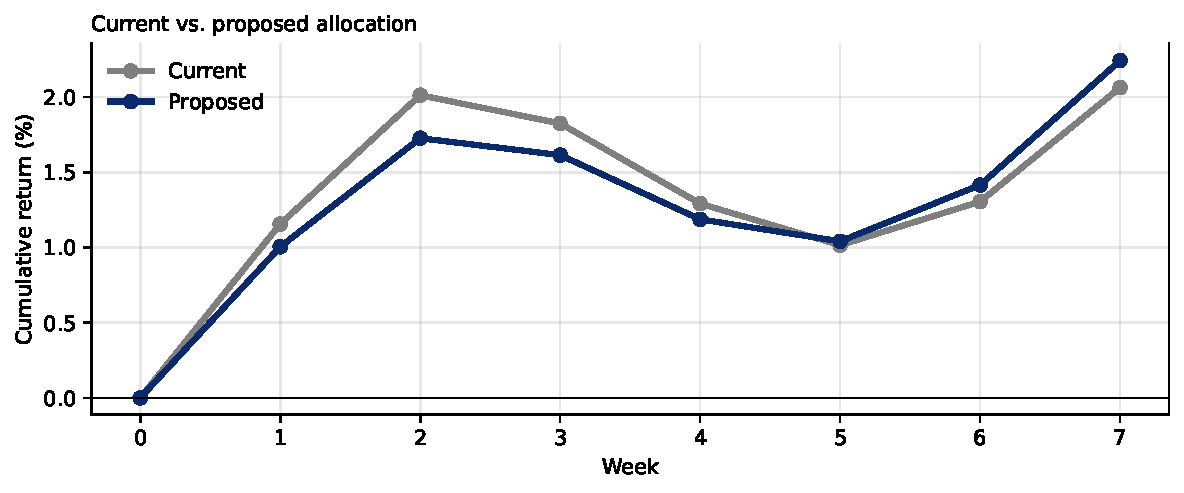
\includegraphics[width=0.85\linewidth]{figures/fig3_allocation.pdf}\par
  {\small\color{gray}Figure 3 --- Cumulative return of the current and proposed
  allocations.}
\end{center}

% ================= Risks =================
\heading{Key Risks to Monitor}
\begin{itemize}[leftmargin=1.5em, itemsep=2pt]
  \item \textbf{Further rate hikes:} would keep pressure on technology
  valuations --- the main reason to reduce the position now.
  \item \textbf{A rate reversal:} if rates start to fall, energy would likely
  weaken; this is why the energy position is kept at 5\%.
  \item \textbf{Earnings and event risk:} technology earnings and geopolitical
  shocks drove the week 3--4 sell-off; the event hedges and cash reserve are
  designed for these moments.
  \item \textbf{Healthcare regulation:} no negative impact in this period, but
  policy changes should be monitored given the 30\% allocation.
  \item \textbf{Limits of the analysis:} seven weeks of data is a short
  sample; the figures show the direction of the effects, not a forecast. The
  analysis should be refreshed as new data arrives.
\end{itemize}

% ================= Closing =================
\heading{Closing Remarks}
Emerald Investments' portfolio is well positioned for long-term growth, and
healthcare has proven its value as a stabiliser. The recent period, however,
showed that the portfolio's short-term volatility is driven almost entirely by
technology. By trimming technology into strength, adding financials and a
small energy position, and turning the cash reserve into a rule-based
opportunity fund, the client keeps its growth engine while making the
portfolio more resilient to rate moves and event shocks.

\textbf{Next steps:} we propose a follow-up meeting to confirm the target
allocation and rebalancing rules, followed by implementation in two stages over
the coming month, and a quarterly review of the portfolio against these
targets.

% ================= Methodology =================
\heading{Appendix: Methodology}
{\small
\begin{itemize}[leftmargin=1.5em, itemsep=1pt]
  \item \textbf{Data:} weekly sector returns, interest rate, VIX, sentiment
  and events for weeks 1--7 (simulation sample dataset).
  \item \textbf{Cumulative returns} are compounded weekly; \textbf{volatility}
  is the sample standard deviation of weekly returns; \textbf{maximum
  drawdown} is the largest fall from a previous high.
  \item \textbf{Risk share} is each holding's contribution to portfolio
  variance, $w_i(\Sigma w)_i / w^\top\Sigma w$, using the sample covariance
  matrix of weekly returns.
  \item \textbf{Cash} earns the weekly equivalent of the prevailing interest
  rate (rate / 52).
  \item All calculations, figures and tables are produced by
  \texttt{analysis.ipynb} in the same folder.
\end{itemize}}

\end{document}
